\chapter{Preserving an ending strategy under safe continuation}\label{ch:endinganalysis}

A system may remain within a declared safe region indefinitely and still lose every way to end its operation. Conversely, an authorized ending procedure may exist at the present state but become unavailable after the next ordinary action. These are distinct requirements. The relevant mathematical object is therefore not a safety invariant alone, but a safe-running region entirely contained in a sure-ending region.

The following development expands the finite result stated earlier in Chapter~\ref{ch:shared}. It supplies an explicit rank proof, treats strategies that depend on observed history, and separates deadlock from an infinite unsuccessful path. Formal correspondence is recorded in the appendix.

\section{Finite game data and the command boundary}
Fix a finite, fully observed configuration set $Z$. Each $z\in Z$ has finite collections $A_{\rm run}(z)$ of running actions and $A_{\rm end}(z)$ of ending actions. For each admitted action $a$ there is a nonempty set $\operatorname{Post}(z,a)\subseteq Z$ of possible successors. A controller chooses an action \emph{before} the successor is determined. The quantifier over all successors is adversarial and is stronger than an expected-value objective.

Let $S\subseteq Z$ be a safe set and $G\subseteq S$ an ending target. At every state of $G$, a hold operation with successors contained in $G$ is available after ending. Running forever means that the controller can choose an admitted action at every pre-command epoch. Deadlock is not counted as successful indefinite operation. A stop command is authenticated and observed before the next action is selected. Whether such an authentication protocol exists in an external institution is not proved by the game calculation. It is part of the model supplied to this theorem.

A strategy may inspect the finite history of observed states and chosen actions. Before the stop command it selects running actions. After the command it selects ending actions. The desired guarantee consists of two clauses: every running path without a command remains safe forever, and every path following a command at any decision epoch reaches $G$ in finitely many ending steps while remaining safe. The strategy must satisfy both clauses under the same command-conditioned policy.

\section{The sure-ending attractor}
Define
\begin{align*}
T_0&=G,\\
T_{k+1}&=T_k\cup\left\{z\in S:\text{some }a\in A_{\rm end}(z)
\text{ satisfies }\operatorname{Post}(z,a)\subseteq T_k\right\}.
\end{align*}
The sequence is increasing and every term is contained in $S$. Because the state set is finite, it becomes constant after finitely many strict additions. Let $T_*$ denote its stable value. For $z\in T_*$, define the first-entry rank $\rho(z)$ as the least $k$ with $z\in T_k$.

\begin{lemma}[Finite-horizon ending criterion]\label{r:end-horizon}
A configuration $z$ belongs to $T_k$ exactly when there exists an ending-only strategy that, whatever the successors, reaches $G$ within at most $k$ transitions while remaining in $S$. In particular, if $\rho(z)>0$, there is an ending action whose every successor has strictly smaller first-entry rank.
\end{lemma}
\begin{proof}
The assertion at $k=0$ says precisely that the initial state is already in $G$. Assume it holds for $k$. If $z\in T_{k+1}\setminus T_k$, the construction supplies an ending action with all successors in $T_k$. After the action the controller uses the strategy given by induction for the observed successor. Every path reaches $G$ within another $k$ transitions. States already in $T_k$ retain their strategy. Conversely, a policy that reaches $G$ in at most $k+1$ steps must either start in $G$, or select some first ending action such that the continuation from every possible successor reaches $G$ within $k$ steps. By induction every such successor belongs to $T_k$, hence the initial state lies in $T_{k+1}$. At the first-entry stage $\rho(z)$, the selected action sends every successor into $T_{\rho(z)-1}$, establishing strict rank decrease.
\end{proof}

\begin{lemma}[Adversarial completeness of the ending region]\label{r:ending-complete}
From a configuration outside $T_*$, no strategy, including one depending on arbitrary finite observed history, can guarantee safe eventual arrival at $G$ along every successor path.
\end{lemma}
\begin{proof}
If the initial configuration is outside $S$, safety has already failed. Otherwise, because $T_*$ is a fixed point, no ending action at a state $z\in S\setminus T_*$ can have all its successors in $T_*$. An adversary can therefore select a successor outside $T_*$ after every proposed ending action. If the selected successor is outside $S$, safety fails. If it remains within $S\setminus T_*$, the same argument can be repeated. The adversary does not need to know the controller's future choices, only its chosen action at each current state. If the controller reaches a non-goal state with no ending action, it deadlocks before reaching the target and loses. Otherwise, either safety fails at a finite step or an infinite path never reaches $G$, which is contained in $T_*$. This defeats any sure-ending guarantee. The argument permits history-dependent policies and requires nonempty successor sets so that the proposed actions represent actual transitions.
\end{proof}

These lemmas show that $T_*$ is not merely the region reached by a convenient algorithm. It is \emph{exactly} the set from which an ending strategy can guarantee success under all modeled successor choices. The rank bounds the required ending transitions by a finite number no greater than the number of strict expansion rounds.

\section{A safety invariant that retains the ending region}
The ending region is not necessarily closed under ordinary running. Define the decreasing sequence
\[
L_0=T_*,\qquad
L_{k+1}=\left\{z\in L_k:\exists a\in A_{\rm run}(z),\ \operatorname{Post}(z,a)\subseteq L_k\right\}.
\]
Let $L_*$ be its stable value. Each stage removes states for which ordinary operation cannot be guaranteed to remain in the preceding stage.

\begin{lemma}[Greatest controlled invariant inside the ending region]\label{r:running-invariant}
The set $L_*$ is the greatest subset of $T_*$ admitting a running action at every member with all successors again in that subset. A state belongs to $L_k$ exactly when a strategy can safely take $k$ running actions while leaving a sure-ending strategy available at every reached decision epoch, including the initial one.
\end{lemma}
\begin{proof}
The bounded-horizon claim follows by induction. At horizon zero only membership in $T_*$ is needed. For the next step, a first running action must send every successor to a state that permits the remaining $k$ running steps and an ending option at every intermediate epoch. Truncating a successful $(k+1)$-step strategy after $k$ steps also shows that its initial state lies in $L_k$. Thus the initial state and all successors of its first action lie in $L_k$, exactly as required by $L_{k+1}$. Conversely, membership supplies the first action and the inductive strategies from its successors.

At stabilization, the defining equation gives one running action for each state in $L_*$ whose successors stay in $L_*$. Selecting these actions proves controlled invariance. If $B\subseteq T_*$ is any other subset with the same property, induction shows $B\subseteq L_k$ for every $k$: inclusion at zero is given. The witnessing running action for any $z\in B$ has all successors in $B\subseteq L_k$, so $z\in L_{k+1}$. Thus $B\subseteq L_*$. No larger controlled invariant within $T_*$ exists.
\end{proof}

\begin{theorem}[Safe running with an available ending at every epoch]\label{r:joint-ending}
A state $z$ belongs to $L_*$ if and only if a single command-conditioned policy can run safely forever in the absence of a command and, upon receiving an authentic stop command at any decision epoch, can reach $G$ on every possible successor path using only ending actions. The stopping phase from a state $w$ reaches $G$ within $\rho(w)$ transitions. The combined policy can be chosen positional in the pair consisting of the current state and the command mode.
\end{theorem}
\begin{proof}
For sufficiency, at each running state in $L_*$ choose an action with all successors in $L_*$. Such actions exist by the preceding lemma and keep every running path within $L_*\subseteq T_*\subseteq S$ for any duration. If a stop command arrives at a decision epoch, the current state still lies in $T_*$. Switch modes and choose a first-entry-rank-decreasing ending action. The rank is a nonnegative integer, decreases strictly after every ending transition outside $G$, and must reach zero in no more than $\rho(w)$ steps. At rank zero the system is in $G$ and can hold safely. This is one policy with the command as its observable mode switch, not two incompatible policies chosen after seeing a future path.

For necessity, consider any policy with the stated guarantee, including one that depends on the entire available history. The stop command may arrive at the present epoch, so by the adversarial completeness lemma the starting state must belong to $T_*$. It may instead arrive after any number $k$ of running steps. Every state reachable immediately before such a command must therefore remain in $T_*$. The running prefix of length $k$ consequently satisfies the bounded-horizon condition of the preceding lemma, so the initial state is in $L_k$. This holds for every $k$. The decreasing sequence stabilizes on a finite set, hence the state belongs to its eventual value $L_*$. No operation is selected with advance knowledge of which successor an adversary will return.
\end{proof}

\section{A three-state obstruction to naive safety}
Consider the safe configurations $S=\{u,z,g\}$ with ending target $G=\{g\}$. The state $g$ has a hold action in both modes, $z$ has a safe running self-loop but cannot end, and $u$ can end immediately at $g$. Yet the only running action at $u$ moves to $z$. This gives
\[
T_*=\{u,g\},\qquad L_*=\{g\}.
\]
It is possible to end from $u$ now, but not to run from $u$ while retaining the option to end later. The obstruction is about \emph{future control access}, not immediate safety.
\begin{figure}[htbp]\centering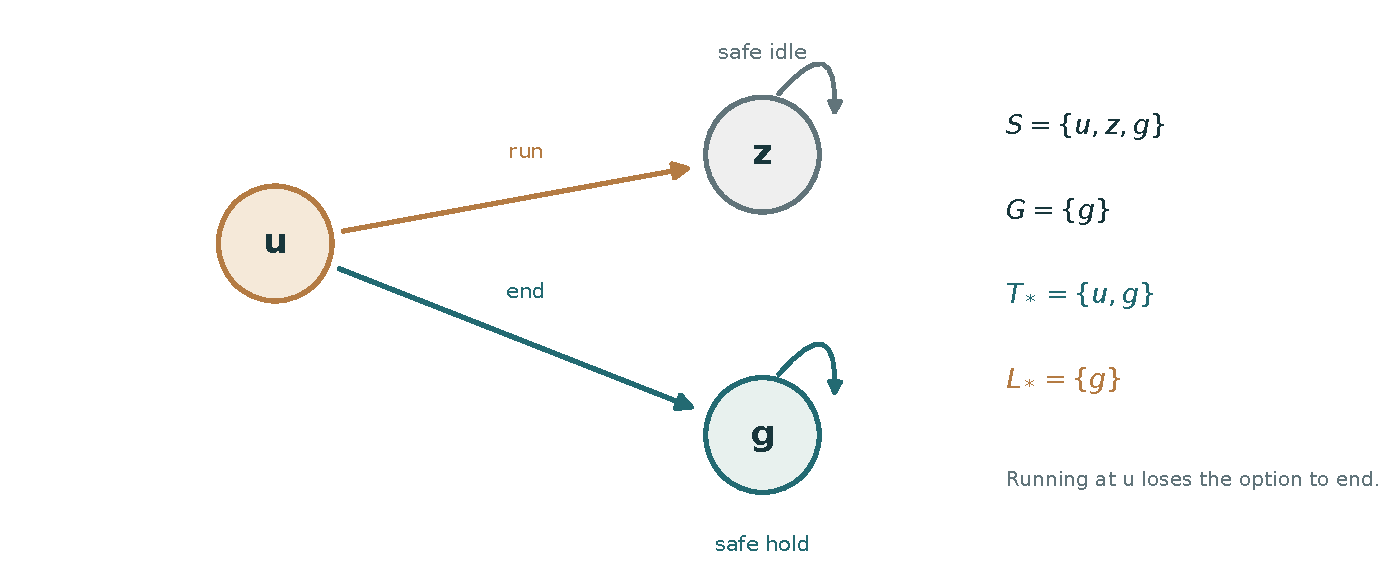
\includegraphics[width=.95\linewidth]{figures/safe_ending_kernel.pdf}\caption{Exact finite safe-running and sure-ending example. The initial running action from $u$ loses the ending option. The sets were checked against explicit strategy enumeration.}\label{fig:ending-kernel}\end{figure}

The companion verifier compares the fixed-point calculation with explicit positional-policy enumeration and checks the rank-decreasing witnesses. The exact input domains and results appear in the verification guide. The calculation treats arrival at $G$ as termination. The stipulated hold concerns subsequent behavior and does not change the reachability calculation.

\section{What changes with partial observation}
The proof assumes the actual configuration is observed when an action is chosen. If only a public report is available, strategies generally act on a belief or possibility state whose update must be justified by the observation protocol. Replacing $Z$ with arbitrary hidden-state names does not produce a valid partially observed ending theorem. One would need a common public-state construction, exact reporting and successor semantics, and a proof that the stop command is observed before action selection. The finite theorem is a solid component of that larger problem without silently solving it.
